% $Id: template.tex 11 2007-04-03 22:25:53Z jpeltier $

\documentclass{vgtc}                          % final (conference style)
\usepackage{authblk}
%\documentclass[review]{vgtc}                 % review
%\documentclass[widereview]{vgtc}             % wide-spaced review
%\documentclass[preprint]{vgtc}               % preprint
%\documentclass[electronic]{vgtc}             % electronic version
\usepackage{amsmath}
\usepackage{algorithm}
% \usepackage{python}
\usepackage{pythontex}
\usepackage[noend]{algpseudocode}

      


\newcommand{\sfunction}[1]{\textsf{\textsc{#1}}}
\algrenewcommand\algorithmicforall{\textbf{foreach}}
\algrenewcommand\algorithmicindent{.8em}

\makeatletter
\def\BState{\State\hskip-\ALG@thistlm}
\makeatother

\ifpdf%                                % if we use pdflatex
  \pdfoutput=1\relax                   % create PDFs from pdfLaTeX
  \pdfcompresslevel=9                  % PDF Compression
  \pdfoptionpdfminorversion=7          % create PDF 1.7
  \ExecuteOptions{pdftex}
  \usepackage{graphicx}                % allow us to embed graphics files
  \DeclareGraphicsExtensions{.pdf,.png,.jpg,.jpeg} % for pdflatex we expect .pdf, .png, or .jpg files
\else%                                 % else we use pure latex
  \ExecuteOptions{dvips}
  \usepackage{graphicx}                % allow us to embed graphics files
  \DeclareGraphicsExtensions{.eps}     % for pure latex we expect eps files
\fi%

%% it is recomended to use ``\autoref{sec:bla}'' instead of ``Fig.~\ref{sec:bla}''
\graphicspath{{figures/}{pictures/}{images/}{./}} % where to search for the images

\usepackage{microtype}                 % use micro-typography (slightly more compact, better to read)
\PassOptionsToPackage{warn}{textcomp}  % to address font issues with \textrightarrow
\usepackage{textcomp}                  % use better special symbols
\usepackage{mathptmx}                  % use matching math font
\usepackage{times}                     % we use Times as the main font
\renewcommand*\ttdefault{txtt}         % a nicer typewriter font
\usepackage{cite}                      % needed to automatically sort the references
\usepackage{tabu}                      % only used for the table example
\usepackage{booktabs}                  % only used for the table example
%% We encourage the use of mathptmx for consistent usage of times font
%% throughout the proceedings. However, if you encounter conflicts
%% with other math-related packages, you may want to disable it.


%% If you are submitting a paper to a conference for review with a double
%% blind reviewing process, please replace the value ``0'' below with your
%% OnlineID. Otherwise, you may safely leave it at ``0''.
\onlineid{0}

%% declare the category of your paper, only shown in review mode
\vgtccategory{Research}

%% allow for this line if you want the electronic option to work properly
% \vgtcinsertpkg

%% In preprint mode you may define your own headline.
%\preprinttext{To appear in an IEEE VGTC sponsored conference.}

%% Paper title.

\title{Solving the N-Queens Problem Using a Genetic Algorithm}

%\author{ \parbox{3 in}{\centering Jon Shaak*
%         \thanks{*Use the $\backslash$thanks command to put information here}\\
%         Faculty of Electrical Engineering, Mathematics and Computer Science\\
%         University of Twente\\
%         7500 AE Enschede, The Netherlands\\
%         {\tt\small h.kwakernaak@autsubmit.com}}
%         \hspace*{ 0.5 in}
%         \parbox{3 in}{ \centering Dugan Dobbs**
%         \thanks{**The footnote marks may be inserted manually}\\
%        Department of Electrical Engineering \\
%         Wright State University\\
%         Dayton, OH 45435, USA\\
%         {\tt\small pmisra@cs.wright.edu}}
%}
\author[1]{\small Dugan Dobbs}
\author[1]{\small Jon Shaak}

\affil[1]{\footnotesize Department of Computer Science, Texas A\&M University, Corpus Christi, TX 78412, USA}

%%%%%%%%%%%%%%%%%%%%%%%%%%%%%%%%%%%%%%%%%%%%%%%%%%%%%%%%%%%%%%%%%%%%%%%%%%%%%%%%
\abstract{

In this paper, a genetic algorithm is applied to the N-Queens problem to find all possible solutions for a particular N. A solution for the N-Queens problem is defined as a board state in which no queens threaten any other. This means they cannot be in the same diagonal, row, or column as any other queen. The genetic algorithm will use the principles of population, selection, crossover, and mutation which will be covered in more detail in this paper. 

}


\begin{document}

%%%%%%%%%%%%%%%%%%%%%%%%%%%%%%%%%%%%%%%%%%%%%%%%%%%%%%%%%%%%%%%%%%%%%%%%%%%%%%%%
\firstsection{Introduction}

\maketitle
The N-Queens problem began with the 8-Queens puzzle first introduced by chess composer Max Bezzel in 1848. In 1850, Franz Nauck proposed the problem in an issue of Illustrirte Zeitung, a famous German newspaper, and originally asserted that there were 60 solutions to the 8-queens problem (cite here 1).The famous mathematician Carl Friedrich Gauss proposed 76 solutions right before Nauck corrected himself and said there were 92 solutions (cite here 1). The important thing to note here is that it took a couple of years to figure out the total number of solutions. To think of how difficult it was to brute force this problem, there are a total of 4.4 billion possible arrangements of 8 queens on an 8 x 8 chessboard. Now, it is proven that if one can find the fundamental solutions of the problem, then the total number of distinct solutions can be found. For example, the 8 queens problem has 12 fundamental solutions and 80 secondary solutions. It is important to recognize that fundamental solutions are distinct solutions that are not rotations or reflections of each other. Based on this fact, we split these 12 fundamental solutions into rotations and reflections. The first solution can be split into four distinct solutions including itself and its rotations. With the 11 remaining states, it is taken into account their four rotations and reflections. Therefore the solution for the number of states yields 11*8 + 1*4 = 92 total distinct states.\par 
	Now, over a century later, the N-queens problem has become a common puzzle in the field of artificial intelligence, with the first algorithm for solving this problem coming from Edsger Dijkstra in 1972. He demonstrated the power of structured programming, demonstrating his depth-first backtracking algorithm to solve the N-queens problem. While this algorithm is not the most efficient way to solve this problem, it introduced the N-queens problem into the field of artificial intelligence. 
    
    
\section{Problem Definition}
The problem states to find the number of solutions, the number of iterations, and the time elapsed to find all solutions of the N-Queens problem using a genetic algorithm. The goal of this study is to prove the efficacy of using a genetic algorithm over other existing algorithms that are used to solve the N-queens problem such as the backtracking algorithm published by Dijkstra. The algorithm used in this study will use a constant population of board states that are randomly generated, a fitness function utilizing the maximum number of attacks a state can achieve as well as the current number of attacks, a tournament selection algorithm paired with a selection probability, a three-way tournament crossover algorithm, and single mutation. Exactly how they are implemented will be further elaborated in the equations and implementations section. The experiment will attempt to limit the iterations and time it takes to find all solutions for any given N.  


\section{Approach}
\subsection{Genetic Algorithms}
A genetic algorithm is a search heuristic inspired by the natural selection theorem of Charles Darwin.It utilizes the main principles of natural selection; those principles being population, selection by fitness, genetic crossover, and genetic mutation. The principles suggest that fit offspring be produced to survive in the environment they are placed in. In the case of a genetic algorithm, fit offspring are created in each generation until the most fit individual in a population is found, a goal state. In the 1960s, John Holland and his colleagues invented genetic algorithms to attempt to formally study the phenomenon of adaptation as it occurs in nature (cite here 2). The other goal of creating a genetic algorithm was to study the mechanisms of natural adaptation and how it could be imported into computer systems (cite here 2). This was a major innovation as many problems in computer programming require programs to be adaptive to changing conditions. \par With problem solving with computers becoming more sophisticated, computer scientists are starting to have a hard time programming problems algorithmically, meaning there are heuristics that are too difficult to compensate for. However, with the innovation of genetic algorithms, the algorithm can adapt to constantly changing environments by creating new "child" states that have acquired better genes than its parents to survive and reproduce until the goal is found. \par There are five phases of a genetic algorithm, the population, fitness function, selection, crossover, and mutation.\\ 

\subsubsection{Population} 
The population is defined by the program designer and should be an optimum amount. If the population is too small, the algorithm will take too much time finding solutions. If the population is too large, the algorithm will also take too long to determine which states are fit to reproduce.\\ 

\subsubsection{Fitness}
The fitness function is determined by the programmer as well depending on the problem they are trying to solve. The function should use a value that represents the most unfit individual state possible and compare the current state's fitness value with the most unfit. The greater the difference between the current state's fitness and the most unfit state's fitness, the more fit the current state actually is.\\ 

\subsubsection{Selection}
Selection determines a probability threshold that determines a state to be selected or not. If the state's fitness does not exceed the probability threshold, it will not be selected as a parent to produce offspring for the next generation.\\ 

\subsubsection{Crossover}
Crossover determines what alleles will be passed on to the child. The child will inherit its alleles from the parent, creating a child with a combination of the two parents, but not being the same as either parent.\\ 

\subsubsection{Mutation} 
Mutation occurs when a random probability the child will mutate matches or exceeds the probability that it will mutate. When this probability is met, the child will have some of its alleles mutate at random that could potentially make it a stronger or weaker state. 

\subsection{March Madness Selection-Tournament}
The proposed March Madness selection tournament is inspired by the March Madness basketball tournament structure. This is a single elimination bracket that start with a power of two number of teams, and ends with one winner. A simple four team bracket example is included in figure \ref{fig:Tournament}. To begin with, the teams are sorted into best-worst pairings. This means that the teams are sorted by fitness, then they are paired with their compliments at the end. In an array structure, the first tier of tournaments are run with teams [1] and [4], then teams [2] and [3]. In terms of n population size, this could be viewed as the psudocode given in algorithms \ref{setup}-\ref{madness}

\begin{figure}
  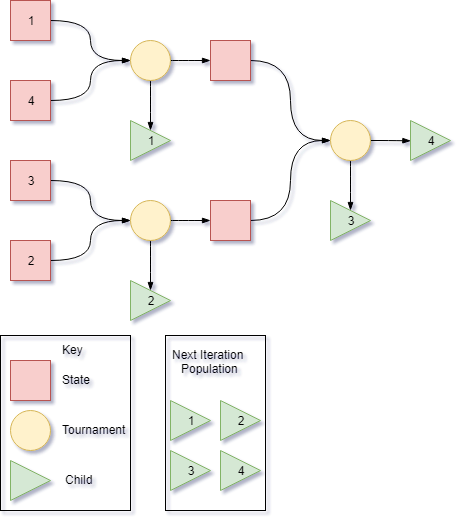
\includegraphics[width=8cm]{Pictures/TournamentFig.png}
  \label{fig:Tournament}
  \caption{Sample Tournament With Population of 4}
\end{figure}

\begin{algorithm}
  \caption{Tournament Setup}\label{setup}
  \begin{algorithmic}[1]
  \Procedure{MarchMadnessRunner}{$n,bSize$}
    \State $populationSize \gets 2^x$
    \State $solutions \gets []$
    \State $population \gets \textit{generatePops}(x)$
    \While{$size(solutions) < totalSolutions$}
      % Generate Fitness
      \State $fitness \gets GenerateFitness(n,bSize,population)$
      % Sort Population, check for finished state, 
      \State $sortedPairs \gets PairAndSort(n,population,fitness)$
      \For{$x \gets 0; x < populationSize; x++$}
        \If{$sortedPairs[x].fitness ==$ $\binom{bSize}{2}$}
          \State $append(solutions,sortedPairs[x].pop)$
         \Else
          \State break
        \EndIf
      \EndFor
      % Send pop,fitness pairs to tournament
      \State $population \gets MMTournament(sortedPairs)$
      % Receive children
    \EndWhile
  \EndProcedure
  \end{algorithmic}
\end{algorithm}

\begin{algorithm}
  \caption{Fitness Generation}\label{Fitness}
  \begin{algorithmic}[1]
  	\Procedure{FitnessGeneration}{$n,bSize,population$}
    \State $fitness \gets []$
      \For{$x \gets 0 ; x < 2^n ; x++$}
        \State $popFit \gets \binom{bSize}{2} - generateClash(population[x])$
        \State $append(fitness,popFit)$
        %\binom{bSize}{2}$}
        % Receive population
        % For pop in population
        % generate fitness
        % return fitness, pop pairs
      \EndFor
    \State $return fitness$
    \EndProcedure
  \end{algorithmic}
\end{algorithm}

\begin{algorithm}
  \caption{March Madness Tournament}\label{madness}
  \begin{algorithmic}[1]
  	\Procedure{MMTournament}{$n,bSize,population$}
      \While {$\textit{size}(pop) > 1$}
        \State $\textit{n} \gets \text{size}(pop)$
        \State $i \gets \textit{n / 2}$
        
        \For {\textit{x in range}(i)}
          \State $t1 \gets pop[x]$.
          \State $t2 \gets pop[n-x]$.
          \State $child ,winner_x \gets \textit{Tournament}(t1,t2)$
          \State $children_x \gets SingleMutation(child)$
        \EndFor
        
        \State $pop \gets winner$
      \EndWhile
      \State $children_{-1} \gets pop$
      \State $\textit{return children}$
    \EndProcedure
  \end{algorithmic}
\end{algorithm}

\begin{figure}
\begin{pycode}
%Hello Jon. This code won't work in overleaf, but it does on a local install. It displays a board defined by arr. Just slap it in and it'll work.
arr = [0,1,2,3,4,5,6,7]
for row in xrange(len(arr)):
  for col in xrange(len(arr)):
    n = row + col
    if n // 2 == n / 2:
    if arr[row] == col:
      print(r"
\includegraphics[width=2cm]{Pictures/BQWT.jpg}")
    else:
      print(r"
\includegraphics[width=2cm]{Pictures/WT.jpg}")
    else:
    if arr[row] == col:
      print(r"
\includegraphics[width=2cm]{Pictures/WQBT.jpg}")
    else:
      print(r"
\includegraphics[width=2cm]{Pictures/BT.jpg}")
\end{pycode}
\label{fig:board1}
\caption{There is supposed to be a board here...}
\end{figure}

\section{Related Works}
A study performed by Uddalok Sarkar and Sayan Nag uses an adaptive genetic algorithm to solve the n-queens problem. They utilize the same principles as stated in the introduction in their genetic algorithm. They use the same fitness function and similar selection of population than the algorithm that will be discussed in this paper, but the elegant step they take is comparing the offspring to the current population and determining if the offspring is fit enough to survive the next generation. If it is not, the offspring is discarded so that its genetics are not added to the gene pool. The results of their algorithm showed that the algorithm only need to perform 1431 iterations to find all solutions for an N of 25. 

\cite{Sarkar2017} This is a garbage citation, it prevents LaTeX from exploding.

\section{Results}

Starting to copy paste results in, formatting comes later.


%num_sols = [1, 0, 0, 2, 10, 4, 40, 92, 352, 724, 2680, 14200, 73712, 365596, 2279184, 14772512, 95815104, 666090624, 4968057848, 39029188884, 314666222712, 2691008701644, 24233937684440, 227514171973736, 2207893435808352, 22317699616364044, 234907967154122528]

% Board size 4:
% SOLUTION FOUND, 1 of 2 [2 0 3 1]
% TIME: 0
% SOLUTION FOUND, 2 of 2 [1 3 0 2]
% TIME: 0
% Found 1 iterations, 0 seconds, 8192 TOTAL INDIVIDUALS

% Board size 5:
% SOLUTION FOUND, 1 of 10 [4 1 3 0 2]
% TIME: 0
% SOLUTION FOUND, 2 of 10 [0 2 4 1 3]
% TIME: 0
% SOLUTION FOUND, 3 of 10 [2 4 1 3 0]
% TIME: 0
% SOLUTION FOUND, 4 of 10 [3 0 2 4 1]
% TIME: 0
% SOLUTION FOUND, 5 of 10 [1 4 2 0 3]
% TIME: 0
% SOLUTION FOUND, 6 of 10 [0 3 1 4 2]
% TIME: 0
% SOLUTION FOUND, 7 of 10 [2 0 3 1 4]
% TIME: 0
% SOLUTION FOUND, 8 of 10 [3 1 4 2 0]
% TIME: 0
% SOLUTION FOUND, 9 of 10 [1 3 0 2 4]
% TIME: 0
% SOLUTION FOUND, 10 of 10 [4 2 0 3 1]
% TIME: 0
% Found 1 iterations, 0 seconds, 8192 TOTAL INDIVIDUALS

% Board size 6
% SOLUTION FOUND, 1 of 4 [4 2 0 5 3 1]
% TIME: 0
% SOLUTION FOUND, 2 of 4 [3 0 4 1 5 2]
% TIME: 1
% SOLUTION FOUND, 3 of 4 [1 3 5 0 2 4]
% TIME: 1
% Found 4 iterations, 1 seconds, 32768 TOTAL INDIVIDUALS

% 7
% SOLUTION FOUND, 1 of 40 [6 4 2 0 5 3 1]
% ITERATION: 3 TIME: 0
% SOLUTION FOUND, 2 of 40 [4 2 0 5 3 1 6]
% ITERATION: 4 TIME: 1
% SOLUTION FOUND, 3 of 40 [5 1 4 0 3 6 2]
% ITERATION: 4 TIME: 1
% SOLUTION FOUND, 4 of 40 [3 6 4 1 5 0 2]
% ITERATION: 7 TIME: 2
% SOLUTION FOUND, 5 of 40 [4 1 5 2 6 3 0]
% ITERATION: 7 TIME: 2
% SOLUTION FOUND, 6 of 40 [3 5 0 2 4 6 1]
% ITERATION: 12 TIME: 4
% SOLUTION FOUND, 7 of 40 [1 4 2 0 6 3 5]
% ITERATION: 15 TIME: 5
% SOLUTION FOUND, 8 of 40 [5 2 0 3 6 4 1]
% ITERATION: 24 TIME: 8
% SOLUTION FOUND, 9 of 40 [6 1 3 5 0 2 4]
% ITERATION: 28 TIME: 10
% SOLUTION FOUND, 10 of 40 [3 1 6 4 2 0 5]
% ITERATION: 28 TIME: 10
% SOLUTION FOUND, 11 of 40 [2 6 1 3 5 0 4]
% ITERATION: 28 TIME: 10
% SOLUTION FOUND, 12 of 40 [5 2 6 3 0 4 1]
% ITERATION: 28 TIME: 10
% SOLUTION FOUND, 13 of 40 [2 6 3 0 4 1 5]
% ITERATION: 37 TIME: 13
% SOLUTION FOUND, 14 of 40 [0 3 6 2 5 1 4]
% ITERATION: 40 TIME: 14
% SOLUTION FOUND, 15 of 40 [0 5 3 1 6 4 2]
% ITERATION: 41 TIME: 14
% SOLUTION FOUND, 16 of 40 [1 6 4 2 0 5 3]
% ITERATION: 41 TIME: 14
% SOLUTION FOUND, 17 of 40 [2 0 5 3 1 6 4]
% ITERATION: 52 TIME: 19
% SOLUTION FOUND, 18 of 40 [4 6 1 5 2 0 3]
% ITERATION: 54 TIME: 19
% SOLUTION FOUND, 19 of 40 [0 2 4 6 1 3 5]
% ITERATION: 62 TIME: 22
% SOLUTION FOUND, 20 of 40 [1 4 0 3 6 2 5]
% ITERATION: 63 TIME: 23
% SOLUTION FOUND, 21 of 40 [1 4 6 3 0 2 5]
% ITERATION: 67 TIME: 24
% SOLUTION FOUND, 22 of 40 [4 0 3 6 2 5 1]
% ITERATION: 67 TIME: 24
% SOLUTION FOUND, 23 of 40 [4 6 1 3 5 0 2]
% ITERATION: 70 TIME: 25
% SOLUTION FOUND, 24 of 40 [1 3 0 6 4 2 5]
% ITERATION: 71 TIME: 26
% SOLUTION FOUND, 25 of 40 [5 0 2 4 6 1 3]
% ITERATION: 75 TIME: 27
% SOLUTION FOUND, 26 of 40 [4 0 5 3 1 6 2]
% ITERATION: 83 TIME: 30
% SOLUTION FOUND, 27 of 40 [6 3 0 4 1 5 2]
% ITERATION: 92 TIME: 33
% SOLUTION FOUND, 28 of 40 [5 3 1 6 4 2 0]
% ITERATION: 96 TIME: 35
% SOLUTION FOUND, 29 of 40 [1 3 5 0 2 4 6]
% ITERATION: 110 TIME: 40
% SOLUTION FOUND, 30 of 40 [5 3 6 0 2 4 1]
% ITERATION: 121 TIME: 44
% SOLUTION FOUND, 31 of 40 [1 5 2 6 3 0 4]
% ITERATION: 123 TIME: 45
% SOLUTION FOUND, 32 of 40 [6 2 5 1 4 0 3]
% ITERATION: 124 TIME: 45
% SOLUTION FOUND, 33 of 40 [5 2 4 6 0 3 1]
% ITERATION: 164 TIME: 60
% SOLUTION FOUND, 34 of 40 [2 0 5 1 4 6 3]
% ITERATION: 196 TIME: 72
% SOLUTION FOUND, 35 of 40 [3 0 2 5 1 6 4]
% ITERATION: 211 TIME: 77
% SOLUTION FOUND, 36 of 40 [2 5 1 4 0 3 6]
% ITERATION: 227 TIME: 83
% SOLUTION FOUND, 37 of 40 [3 6 2 5 1 4 0]
% ITERATION: 231 TIME: 85
% SOLUTION FOUND, 38 of 40 [2 4 6 1 3 5 0]
% ITERATION: 278 TIME: 102
% SOLUTION FOUND, 39 of 40 [3 0 4 1 5 2 6]
% ITERATION: 382 TIME: 141
% Found 382 iterations, 141 seconds, 3129344 TOTAL INDIVIDUALS

% BOARD SIZE 8
% SOLUTION FOUND, 1 of 92 [3 6 2 7 1 4 0 5]
% ITERATION: 14 TIME: 5
% SOLUTION FOUND, 2 of 92 [4 0 7 3 1 6 2 5]
% ITERATION: 27 TIME: 11
% SOLUTION FOUND, 3 of 92 [3 1 7 4 6 0 2 5]
% ITERATION: 98 TIME: 41
% SOLUTION FOUND, 4 of 92 [2 7 3 6 0 5 1 4]
% ITERATION: 128 TIME: 54
% SOLUTION FOUND, 5 of 92 [6 3 1 7 5 0 2 4]
% ITERATION: 164 TIME: 70
% SOLUTION FOUND, 6 of 92 [0 6 4 7 1 3 5 2]
% ITERATION: 172 TIME: 73
% SOLUTION FOUND, 7 of 92 [2 5 1 4 7 0 6 3]
% ITERATION: 231 TIME: 99
% SOLUTION FOUND, 8 of 92 [6 4 2 0 5 7 1 3]
% ITERATION: 247 TIME: 106
% SOLUTION FOUND, 9 of 92 [5 1 6 0 2 4 7 3]
% ITERATION: 262 TIME: 112
% SOLUTION FOUND, 10 of 92 [5 1 6 0 3 7 4 2]
% ITERATION: 288 TIME: 123
% SOLUTION FOUND, 11 of 92 [5 2 4 6 0 3 1 7]
% ITERATION: 317 TIME: 136
% SOLUTION FOUND, 12 of 92 [2 5 7 1 3 0 6 4]
% ITERATION: 325 TIME: 139
% SOLUTION FOUND, 13 of 92 [3 1 6 4 0 7 5 2]
% ITERATION: 328 TIME: 140
% SOLUTION FOUND, 14 of 92 [4 2 0 5 7 1 3 6]
% ITERATION: 344 TIME: 147
% SOLUTION FOUND, 15 of 92 [2 5 1 6 4 0 7 3]
% ITERATION: 375 TIME: 160
% SOLUTION FOUND, 16 of 92 [2 4 6 0 3 1 7 5]
% ITERATION: 385 TIME: 164
% SOLUTION FOUND, 17 of 92 [3 7 0 4 6 1 5 2]
% ITERATION: 419 TIME: 179
% SOLUTION FOUND, 18 of 92 [6 0 2 7 5 3 1 4]
% ITERATION: 473 TIME: 202
% SOLUTION FOUND, 19 of 92 [7 1 3 0 6 4 2 5]
% ITERATION: 491 TIME: 210
% SOLUTION FOUND, 20 of 92 [1 3 5 7 2 0 6 4]
% ITERATION: 574 TIME: 245
% SOLUTION FOUND, 21 of 92 [5 0 4 1 7 2 6 3]
% ITERATION: 586 TIME: 250
% SOLUTION FOUND, 22 of 92 [7 3 0 2 5 1 6 4]
% ITERATION: 626 TIME: 267
% SOLUTION FOUND, 23 of 92 [5 3 6 0 2 4 1 7]
% ITERATION: 656 TIME: 280
% SOLUTION FOUND, 24 of 92 [2 4 1 7 0 6 3 5]
% ITERATION: 657 TIME: 280
% SOLUTION FOUND, 25 of 92 [7 1 4 2 0 6 3 5]
% ITERATION: 725 TIME: 309
% SOLUTION FOUND, 26 of 92 [3 1 6 2 5 7 4 0]
% ITERATION: 765 TIME: 326
% SOLUTION FOUND, 27 of 92 [4 7 3 0 2 5 1 6]
% ITERATION: 779 TIME: 332
% SOLUTION FOUND, 28 of 92 [6 1 5 2 0 3 7 4]
% ITERATION: 806 TIME: 344
% SOLUTION FOUND, 29 of 92 [3 0 4 7 1 6 2 5]
% ITERATION: 931 TIME: 407
% SOLUTION FOUND, 30 of 92 [5 2 6 1 3 7 0 4]
% ITERATION: 941 TIME: 411
% SOLUTION FOUND, 31 of 92 [2 4 7 3 0 6 1 5]
% ITERATION: 949 TIME: 415
% SOLUTION FOUND, 32 of 92 [3 6 4 1 5 0 2 7]
% ITERATION: 1062 TIME: 465
% SOLUTION FOUND, 33 of 92 [6 2 0 5 7 4 1 3]
% ITERATION: 1071 TIME: 468
% SOLUTION FOUND, 34 of 92 [5 7 1 3 0 6 4 2]
% ITERATION: 1135 TIME: 496
% SOLUTION FOUND, 35 of 92 [5 2 4 7 0 3 1 6]
% ITERATION: 1164 TIME: 508
% SOLUTION FOUND, 36 of 92 [4 1 5 0 6 3 7 2]
% ITERATION: 1207 TIME: 526
% SOLUTION FOUND, 37 of 92 [1 5 7 2 0 3 6 4]
% ITERATION: 1283 TIME: 559
% SOLUTION FOUND, 38 of 92 [4 6 1 3 7 0 2 5]
% ITERATION: 1291 TIME: 562
% SOLUTION FOUND, 39 of 92 [5 3 1 7 4 6 0 2]
% ITERATION: 1347 TIME: 586
% SOLUTION FOUND, 40 of 92 [5 3 6 0 7 1 4 2]
% ITERATION: 1363 TIME: 593
% SOLUTION FOUND, 41 of 92 [5 2 0 7 3 1 6 4]
% ITERATION: 1376 TIME: 598
% SOLUTION FOUND, 42 of 92 [2 5 3 0 7 4 6 1]
% ITERATION: 1384 TIME: 601
% SOLUTION FOUND, 43 of 92 [4 2 0 6 1 7 5 3]
% ITERATION: 1403 TIME: 609
% SOLUTION FOUND, 44 of 92 [1 4 6 3 0 7 5 2]
% ITERATION: 1508 TIME: 654
% SOLUTION FOUND, 45 of 92 [4 1 7 0 3 6 2 5]
% ITERATION: 1588 TIME: 688
% SOLUTION FOUND, 46 of 92 [1 6 4 7 0 3 5 2]
% ITERATION: 1635 TIME: 708
% SOLUTION FOUND, 47 of 92 [4 0 7 5 2 6 1 3]
% ITERATION: 1748 TIME: 758
% SOLUTION FOUND, 48 of 92 [2 5 3 1 7 4 6 0]
% ITERATION: 1757 TIME: 762
% SOLUTION FOUND, 49 of 92 [2 6 1 7 4 0 3 5]
% ITERATION: 1818 TIME: 789
% SOLUTION FOUND, 50 of 92 [6 2 7 1 4 0 5 3]
% ITERATION: 1823 TIME: 791
% SOLUTION FOUND, 51 of 92 [4 1 3 6 2 7 5 0]
% ITERATION: 1859 TIME: 807
% SOLUTION FOUND, 52 of 92 [3 7 0 2 5 1 6 4]
% ITERATION: 1865 TIME: 809
% SOLUTION FOUND, 53 of 92 [3 7 4 2 0 6 1 5]
% ITERATION: 1953 TIME: 847
% SOLUTION FOUND, 54 of 92 [5 3 0 4 7 1 6 2]
% ITERATION: 1955 TIME: 848
% SOLUTION FOUND, 55 of 92 [1 5 0 6 3 7 2 4]
% ITERATION: 1956 TIME: 848
% SOLUTION FOUND, 56 of 92 [6 1 3 0 7 4 2 5]
% ITERATION: 2050 TIME: 888
% SOLUTION FOUND, 57 of 92 [1 4 6 0 2 7 5 3]
% ITERATION: 2192 TIME: 949
% SOLUTION FOUND, 58 of 92 [4 1 3 5 7 2 0 6]
% ITERATION: 2221 TIME: 961
% SOLUTION FOUND, 59 of 92 [4 6 1 5 2 0 7 3]
% ITERATION: 2256 TIME: 976
% SOLUTION FOUND, 60 of 92 [1 6 2 5 7 4 0 3]
% ITERATION: 2291 TIME: 991
% SOLUTION FOUND, 61 of 92 [3 1 6 2 5 7 0 4]
% ITERATION: 2595 TIME: 1121
% SOLUTION FOUND, 62 of 92 [0 4 7 5 2 6 1 3]
% ITERATION: 2887 TIME: 1246
% SOLUTION FOUND, 63 of 92 [5 2 6 1 7 4 0 3]
% ITERATION: 2979 TIME: 1285
% SOLUTION FOUND, 64 of 92 [3 6 0 7 4 1 5 2]
% ITERATION: 2987 TIME: 1289
% SOLUTION FOUND, 65 of 92 [4 6 0 2 7 5 3 1]
% ITERATION: 3050 TIME: 1316
% SOLUTION FOUND, 66 of 92 [4 2 7 3 6 0 5 1]
% ITERATION: 3116 TIME: 1344
% SOLUTION FOUND, 67 of 92 [2 5 7 0 4 6 1 3]
% ITERATION: 3128 TIME: 1349
% SOLUTION FOUND, 68 of 92 [2 0 6 4 7 1 3 5]
% ITERATION: 3190 TIME: 1376
% SOLUTION FOUND, 69 of 92 [4 7 3 0 6 1 5 2]
% ITERATION: 3359 TIME: 1448
% SOLUTION FOUND, 70 of 92 [2 5 1 6 0 3 7 4]
% ITERATION: 3425 TIME: 1476
% SOLUTION FOUND, 71 of 92 [0 6 3 5 7 1 4 2]
% ITERATION: 3442 TIME: 1483
% SOLUTION FOUND, 72 of 92 [3 1 4 7 5 0 2 6]
% ITERATION: 3462 TIME: 1492
% SOLUTION FOUND, 73 of 92 [2 4 1 7 5 3 6 0]
% ITERATION: 3473 TIME: 1497
% SOLUTION FOUND, 74 of 92 [5 2 0 6 4 7 1 3]
% ITERATION: 4047 TIME: 1743
% SOLUTION FOUND, 75 of 92 [3 0 4 7 5 2 6 1]
% ITERATION: 4060 TIME: 1749
% SOLUTION FOUND, 76 of 92 [7 2 0 5 1 4 6 3]
% ITERATION: 4212 TIME: 1814
% SOLUTION FOUND, 77 of 92 [3 5 7 2 0 6 4 1]
% ITERATION: 4258 TIME: 1833
% SOLUTION FOUND, 78 of 92 [5 2 0 7 4 1 3 6]
% ITERATION: 4373 TIME: 1883
% SOLUTION FOUND, 79 of 92 [4 0 3 5 7 1 6 2]
% ITERATION: 4512 TIME: 1942
% SOLUTION FOUND, 80 of 92 [3 6 4 2 0 5 7 1]
% ITERATION: 4646 TIME: 2000
% SOLUTION FOUND, 81 of 92 [3 5 0 4 1 7 2 6]
% ITERATION: 5188 TIME: 2232
% SOLUTION FOUND, 82 of 92 [0 5 7 2 6 3 1 4]
% ITERATION: 5475 TIME: 2355
% SOLUTION FOUND, 83 of 92 [5 2 6 3 0 7 1 4]
% ITERATION: 5479 TIME: 2357
% SOLUTION FOUND, 84 of 92 [4 6 0 3 1 7 5 2]
% ITERATION: 5784 TIME: 2486
% SOLUTION FOUND, 85 of 92 [4 6 1 5 2 0 3 7]
% ITERATION: 5843 TIME: 2511
% SOLUTION FOUND, 86 of 92 [2 6 1 7 5 3 0 4]
% ITERATION: 6253 TIME: 2690
% SOLUTION FOUND, 87 of 92 [1 7 5 0 2 4 6 3]
% ITERATION: 6341 TIME: 2729
% SOLUTION FOUND, 88 of 92 [3 5 7 1 6 0 2 4]
% ITERATION: 7072 TIME: 3046
% SOLUTION FOUND, 89 of 92 [6 3 1 4 7 0 2 5]
% ITERATION: 7391 TIME: 3181
% SOLUTION FOUND, 90 of 92 [4 6 3 0 2 7 5 1]
% ITERATION: 7698 TIME: 3311
% SOLUTION FOUND, 91 of 92 [2 5 7 0 3 6 4 1]
% ITERATION: 8334 TIME: 3581
% Found 8334 iterations, 3581 seconds, 68272128 TOTAL INDIVIDUALS


\section{Discussion}

A conclusion section is not required. Although a conclusion may review the main points of the paper, do not replicate the abstract as the conclusion. A conclusion might elaborate on the importance of the work or suggest applications and extensions. 

\section*{APPENDIX}

Appendixes should appear before the acknowledgment.

\section*{ACKNOWLEDGMENT}



%%%%%%%%%%%%%%%%%%%%%%%%%%%%%%%%%%%%%%%%%%%%%%%%%%%%%%%%%%%%%%%%%%%%%%%%%%%%%%%%

References are important to the reader; therefore, each citation must be complete and correct. If at all possible, references should be commonly available publications.

\bibliographystyle{superstyle}
\bibliography{bib}
% \maxdeadcycles=1000
\end{document}
